% !TeX root = f61_longreport_schmitt_kleinbek.tex
\newpage
\section{Measurements Log and Evaluation}


%------------------------
\subsection{Experimental setup}
The relaxation times and the chemical shift were measured with a Bruker minispec p20 (see fig. \ref{fig:setup}).
\begin{figure}[ht]
\centering
\begin{subfigure}{.45\textwidth}
\centering
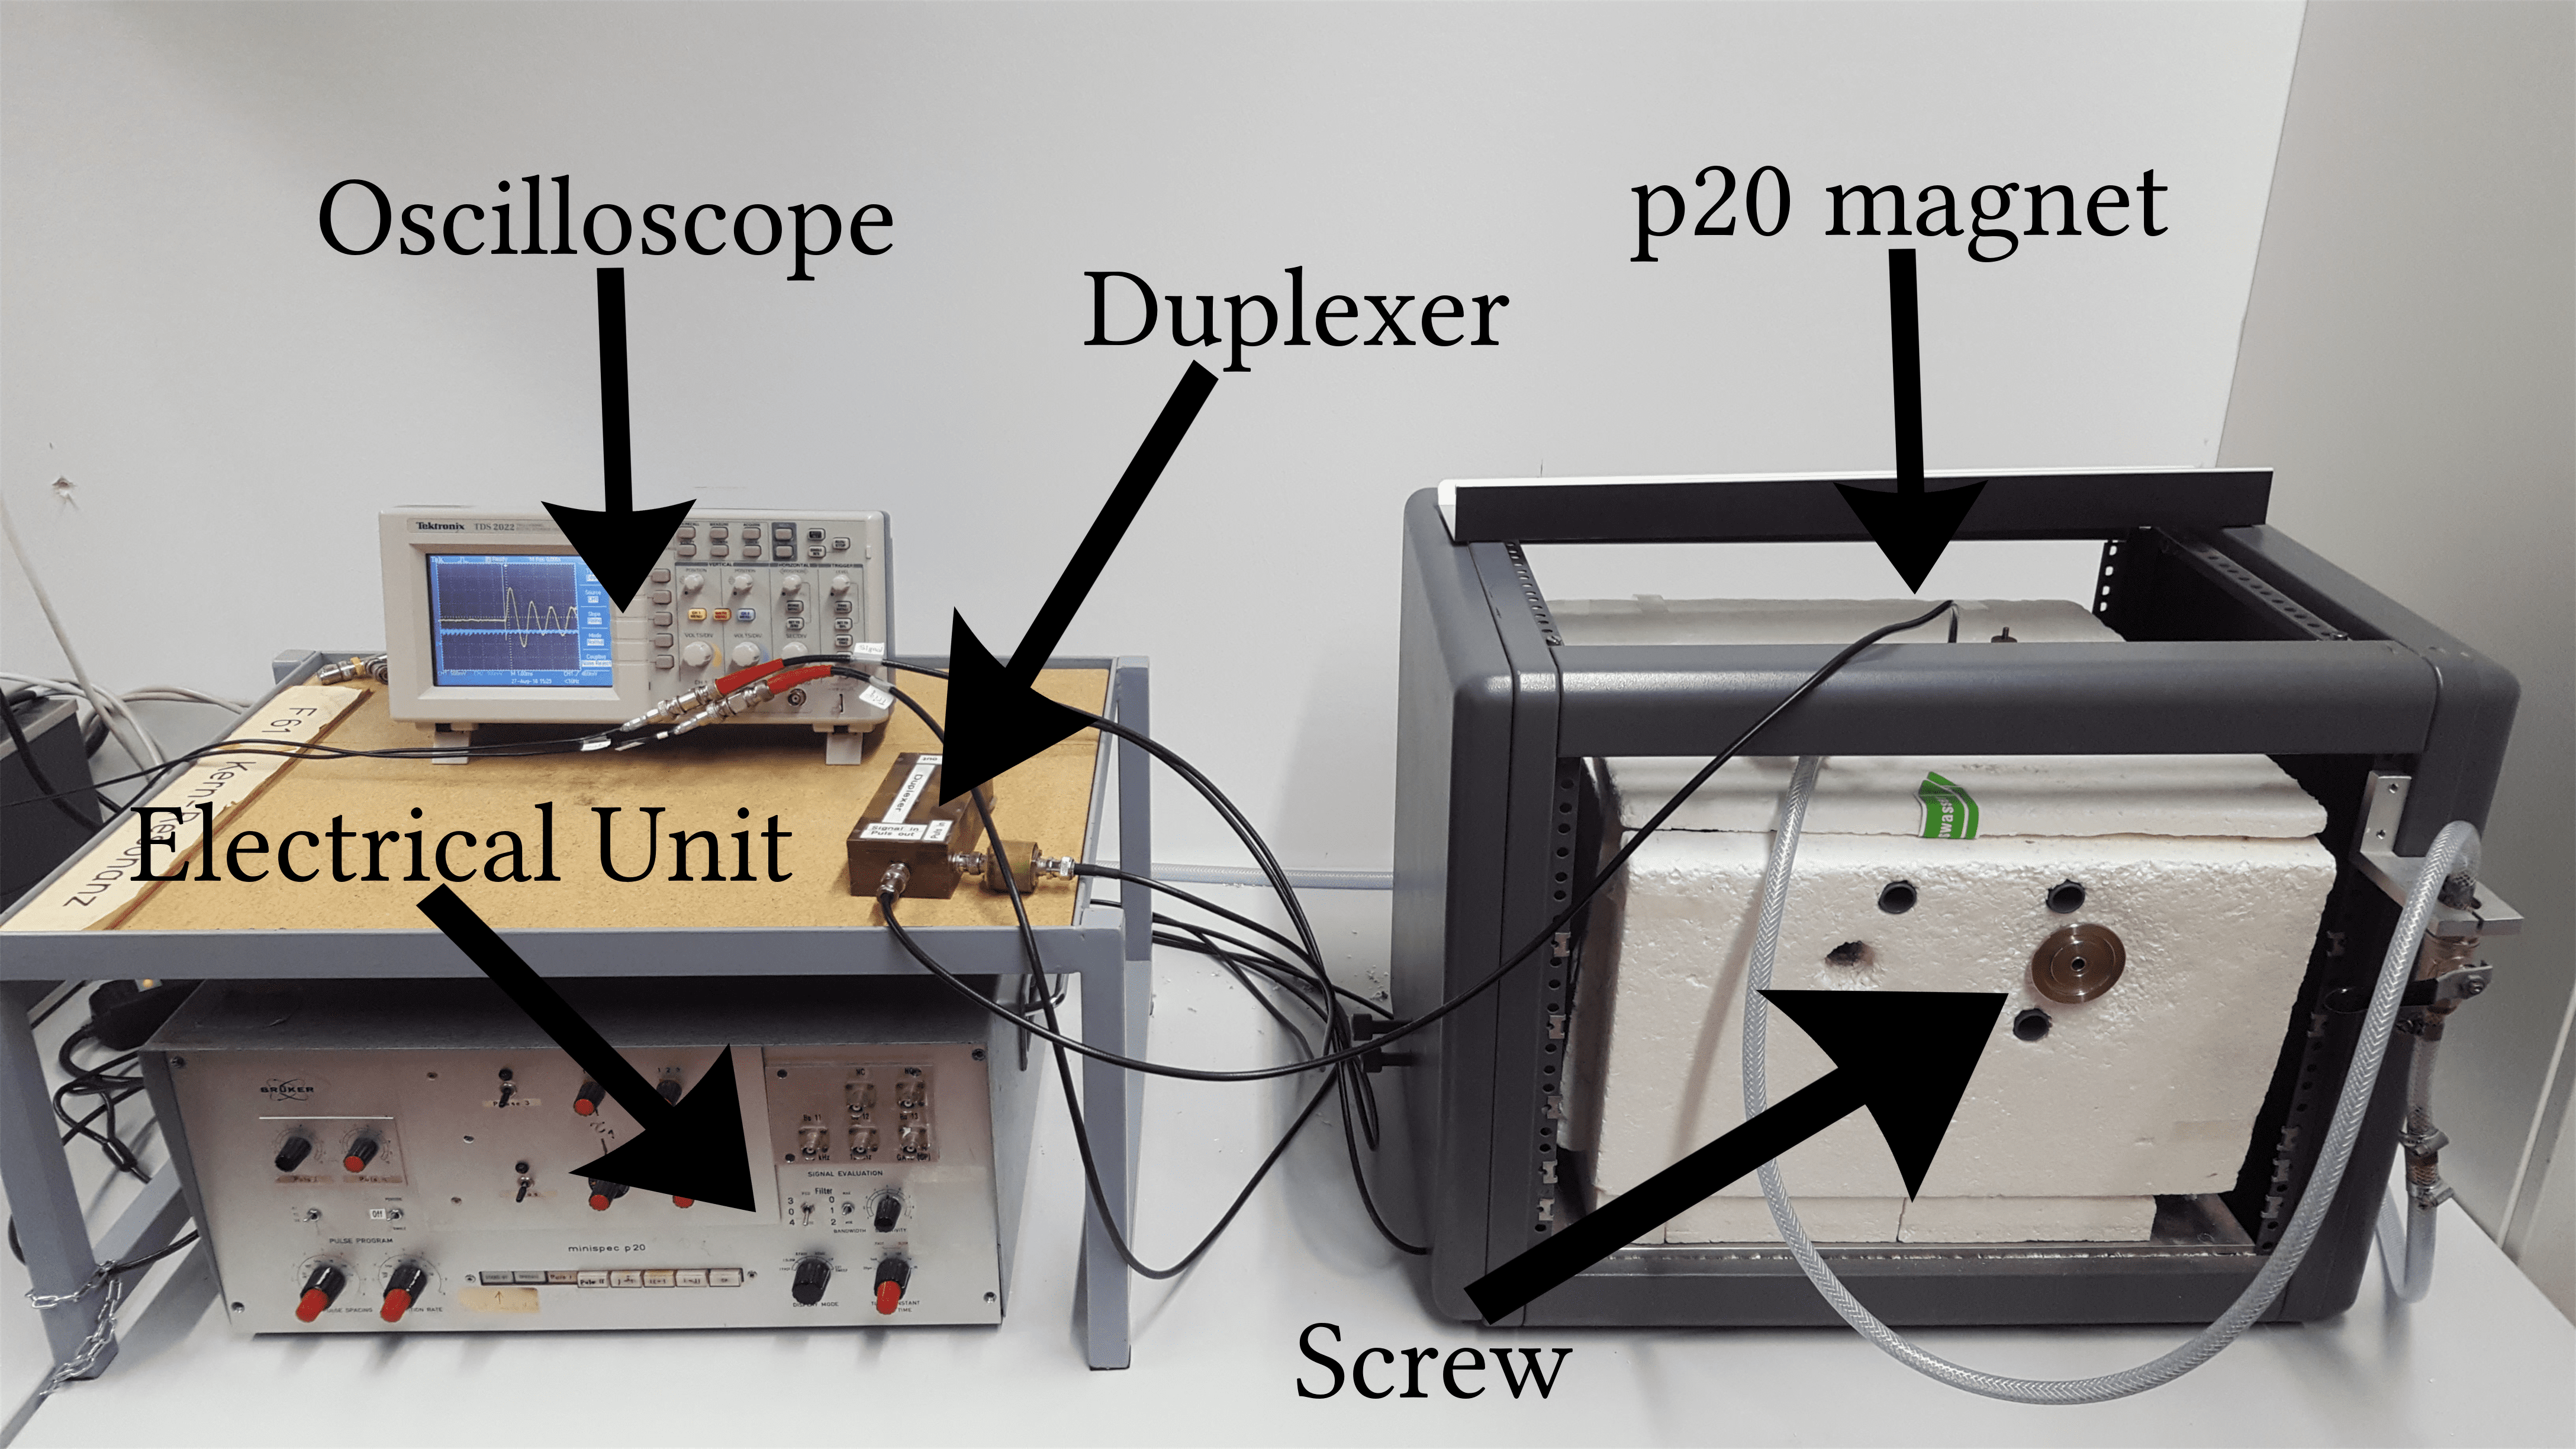
\includegraphics[height =4.5cm]{images//setup.png}
\caption{Entire Configuration}
\end{subfigure}
\quad
\begin{subfigure}{.45\textwidth}
\centering
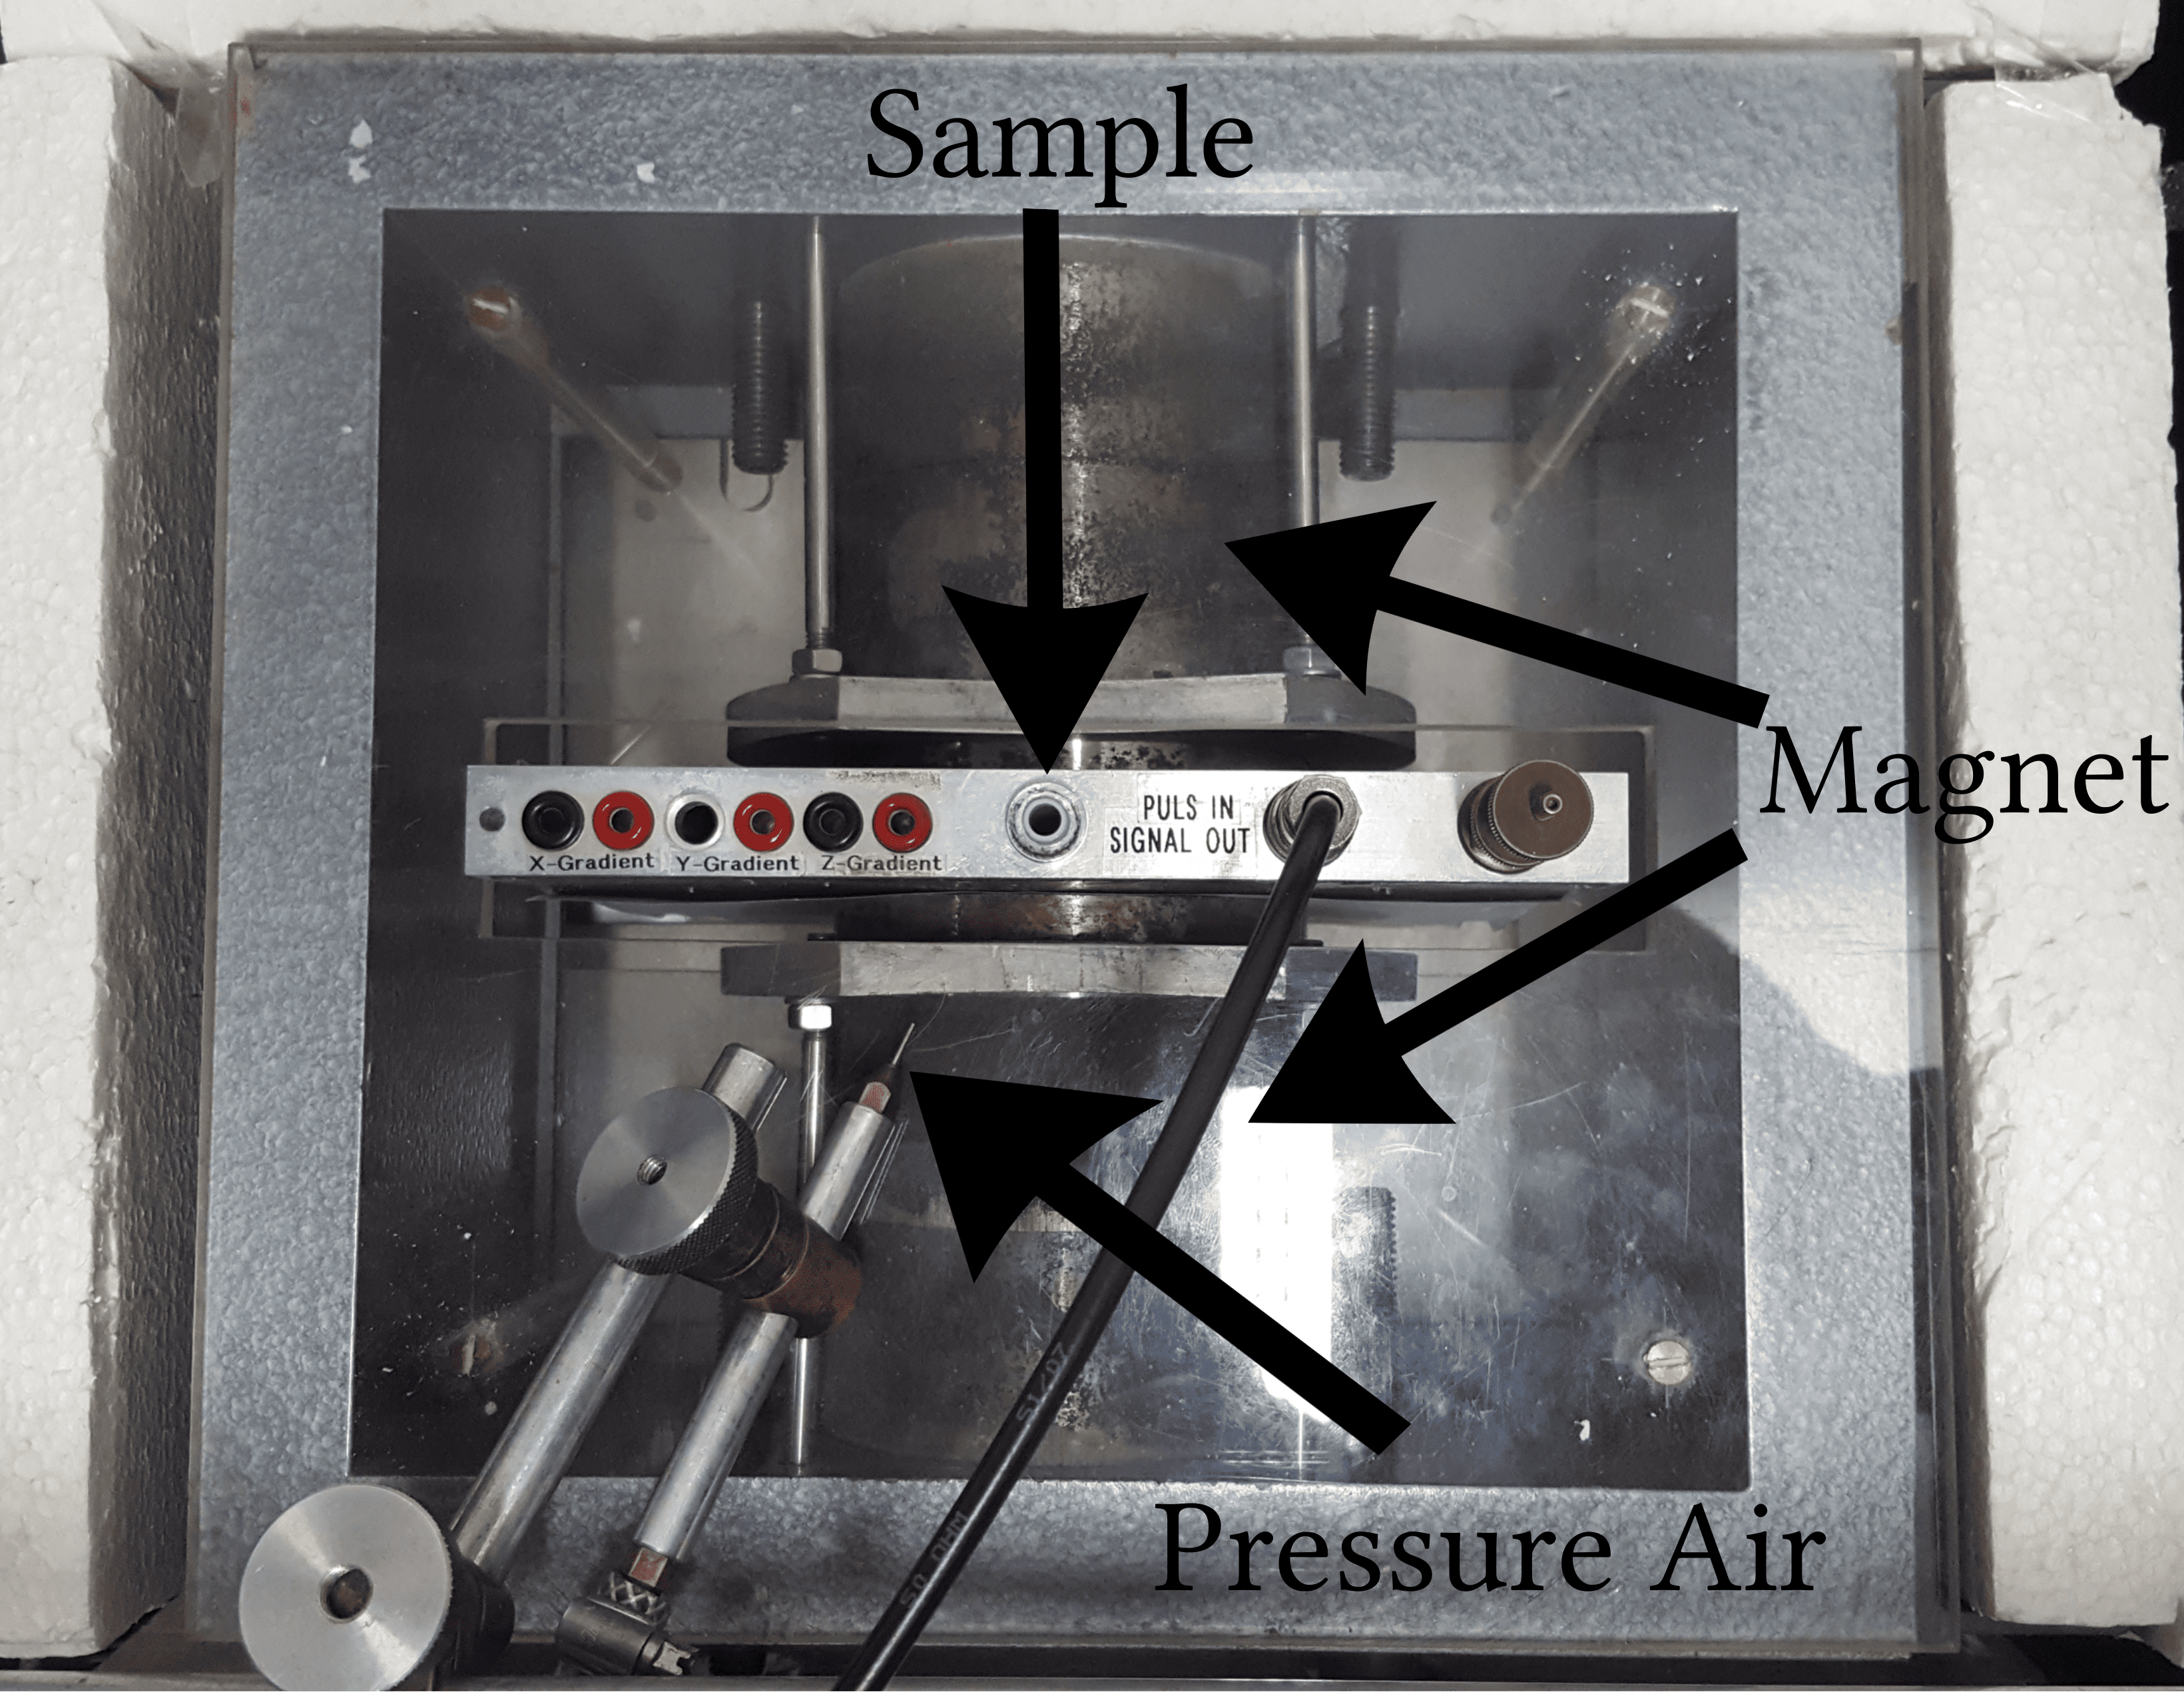
\includegraphics[height=4.5cm]{images//magnet.png}
\caption{p20 magnet}
\end{subfigure}
\caption{Experimental setup.}
\label{fig:setup}
\end{figure}
The arrangement is divided into the p20 electrical unit and the p20 magnet.\\
The electrical unit can generate two different pulses (hereinafter called pulse I and pulse II), as well as I-I, I-II and II-I sequences and a Carr-Purcell sequence.
For the sequences the duration between the individual pulses and for the individual pulses the pulse duration can be set.
The latter was later adjusted so that the two pulses correspond to a $\ang{90}$ or $\ang{180}$ pulse.
The signal generated by the electrical unit is conducted into the magnet, where it generates a magnetic field that deflects the magnetic moments of the atomic nuclei in the sample.
These rotate as described in the previous section with the Larmor frequency and generate a signal with this frequency in an induction coil inside the structure.
This signal is fed back into the electronic unit via the duplexer, where it is modulated with the high-frequency excitation frequency.
The resulting signal has an working frequency which indicates the difference between the excitation frequency and the Larmor frequency.
This is displayed on the oscilloscope and read out and evaluated on the PC with LabView.


%------------------------
\subsection{Determination of relaxation time}

\subsubsection{Spin-spin interaction $T_2$ using spin-echo method}
As described in the theoretical principles, different time spans $\tau$ were set as the interval duration between the $\ang{90}$ pulse and the $\ang{180}$ pulse and the intensity of the observed echo was measured after each period of $2\tau$, when all spins again contributed in phase to a maximum induction current.\\
When measuring the Gd500 sample we regularly checked the working frequency values and found that this value increased from initially $\omega_f=\SI{900(40)}{\hertz}$ to now $\omega_f=\SI{1150(20)}{\hertz}$ and finally to $\omega_f=\SI{1170(20)}{\hertz}$.
The reason for this is a change in the Larmor frequency of the hydrogen atoms due to a change in the external magnetic field $B_0$, which is caused by temperature fluctuations in the laboratory.
Although we tried to check the working frequency regularly and correct any deviations with the screw shown above, this inconsistency of the working frequency has effects on our measurement results that have yet to be discussed.\\

If echo times are too high, diffusion change the position of the atoms so the are no longer all in phase again at the corresponding echo time.
This effect reduces the intensity of the echo signal by independent migration and change of the magnetic field.\\
The results of the measurement for the Gd500 sample and the equivalent Gd600 sample are plotted with Python in Figure \ref{fig:t2se} and provided with an exponential fit according to equation \ref{eq:t2}.
\begin{figure}[ht]
\begin{subfigure}{.45\textwidth}
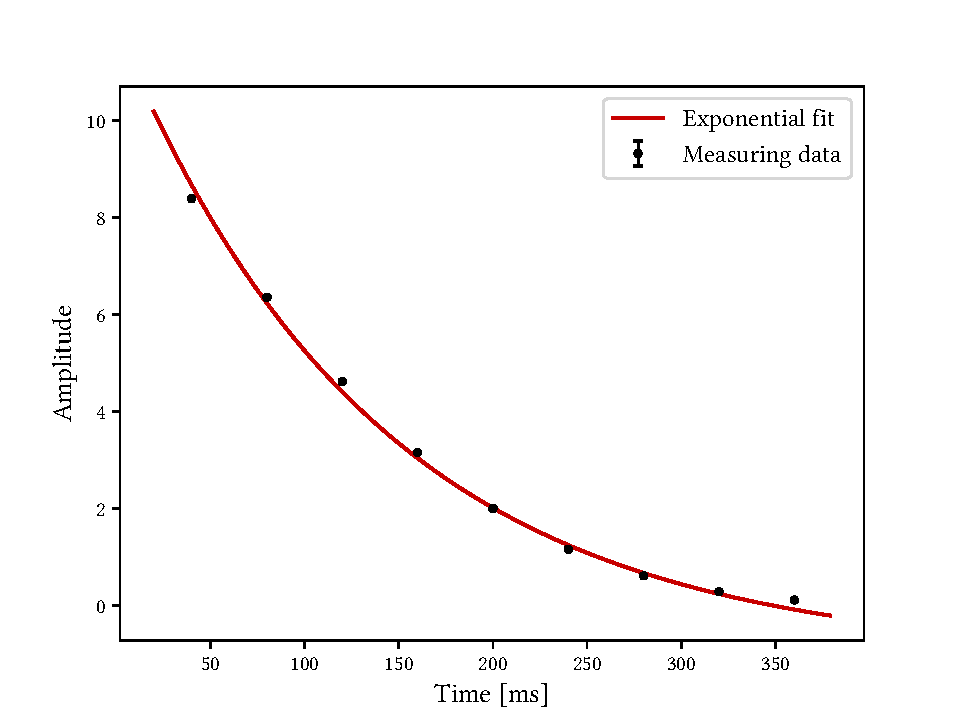
\includegraphics[width=9.3cm]{..//figures//f61_abb_2.pdf}
\caption{Gd500}
\end{subfigure}
\qquad
\begin{subfigure}{.45\textwidth}
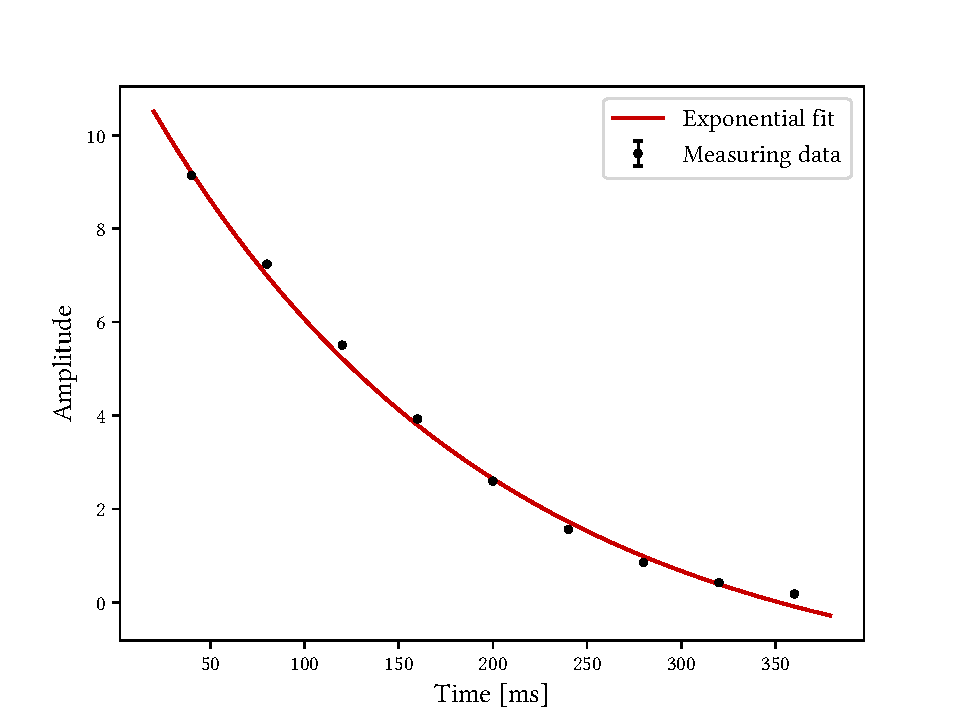
\includegraphics[width=9.3cm]{..//figures//f61_abb_2_600.pdf}
\caption{Gd600}
\end{subfigure}
\caption{Results of the measurement for relaxation time $T_2$ using spin-echo method}.
\label{fig:t2se}
\end{figure}
This way we get the relaxation times
\begin{align*}
T_{2,\text{ Gd500},\text{ spin-echo}}&=\SI{154.2(9)}{\milli\second},\\
T_{2,\text{ Gd600},\text{ spin-echo}}&=\SI{186.5(9)}{\milli\second}
\end{align*}
for our measurement.

\subsubsection{Spin-spin interaction $T_2$ using Carr-Purcell method}
The only difference between the Carr-Purcell method and the previous spin-echo method is the recurring $\ang{180}$ pulse, so that echo signals appear again and again at intervals of $2\tau$ and the exponential decrease in amplitude can already be seen in one signal.\\
Because the values are recorded directly one after the other and possible inconsistencies in the magnetic field or other parts of the test setup do not have such a large influence, the results of the Carr-Purcell series of measurements appear more credible.\\
After the Python fit we get the values
\begin{align*}
T_{2,\text{ Gd500},\text{ Carr-Purcell}}&=\SI{170.1(4)}{\milli\second},\\
T_{2,\text{ Gd600},\text{ Carr-Purcell}}&=\SI{198.2(7)}{\milli\second}
\end{align*}
from figure \ref{fig:t2cp}.
\begin{figure}[ht]
\begin{subfigure}{.45\textwidth}
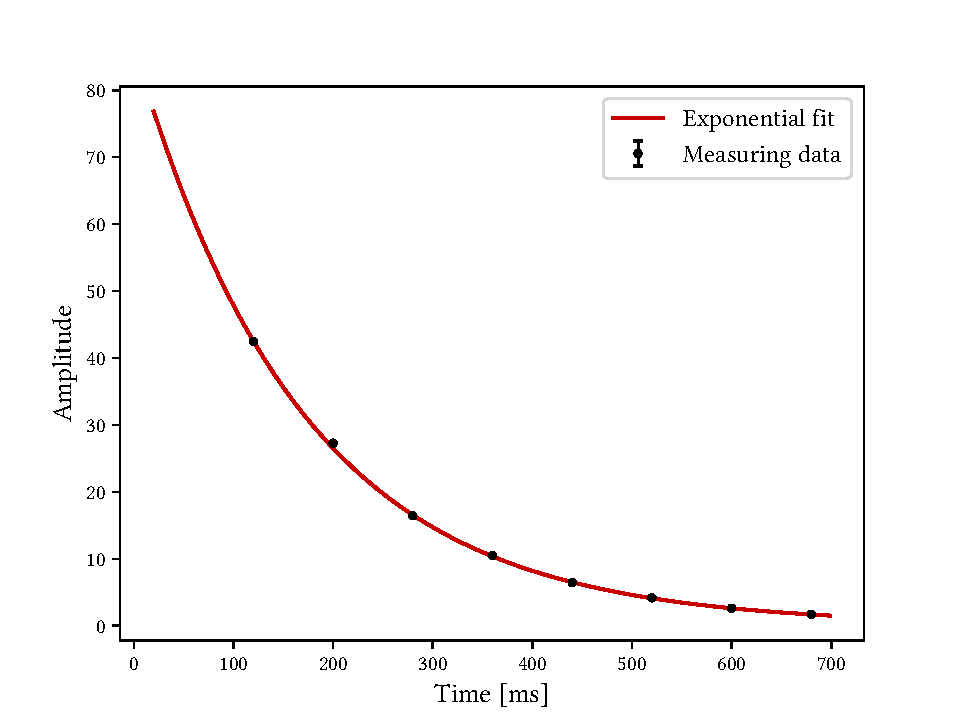
\includegraphics[width=9.3cm]{..//figures//f61_abb_3.pdf}
\caption{Gd500}
\end{subfigure}
\qquad
\begin{subfigure}{.45\textwidth}
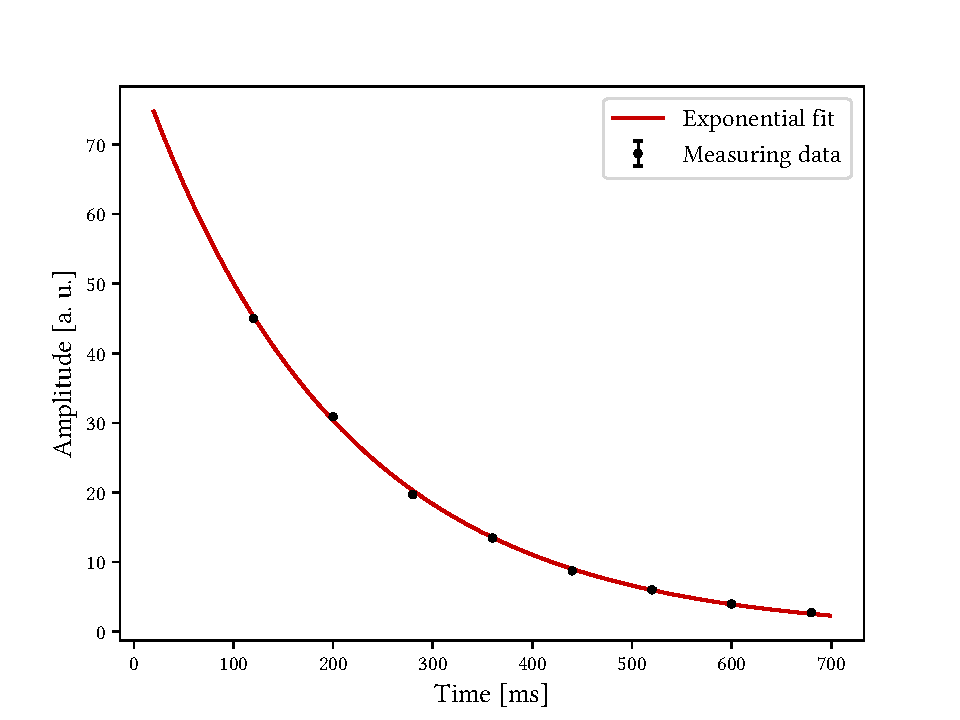
\includegraphics[width=9.3cm]{..//figures//f61_abb_3_600.pdf}
\caption{Gd600}
\end{subfigure}
\caption{Results of the measurement for relaxation time $T_2$ using Carr-Purcell sequence.}
\label{fig:t2cp}
\end{figure}

\subsubsection{Spin-lattice interaction $T_1$}
With the sequence of $\ang{180}$ and $\ang{90}$ pulses described in the basics after different times and respective intensity measurement of the signal after this time, the increase of magnetization in the direction of the magnetic field can be measured.\\
The corresponding plots for the relaxation time of the spin-lattice interaction $T_1$ for both gadolinium samples are shown in figure \ref{fig:t1}.
\begin{figure}[ht]
\begin{subfigure}{.45\textwidth}
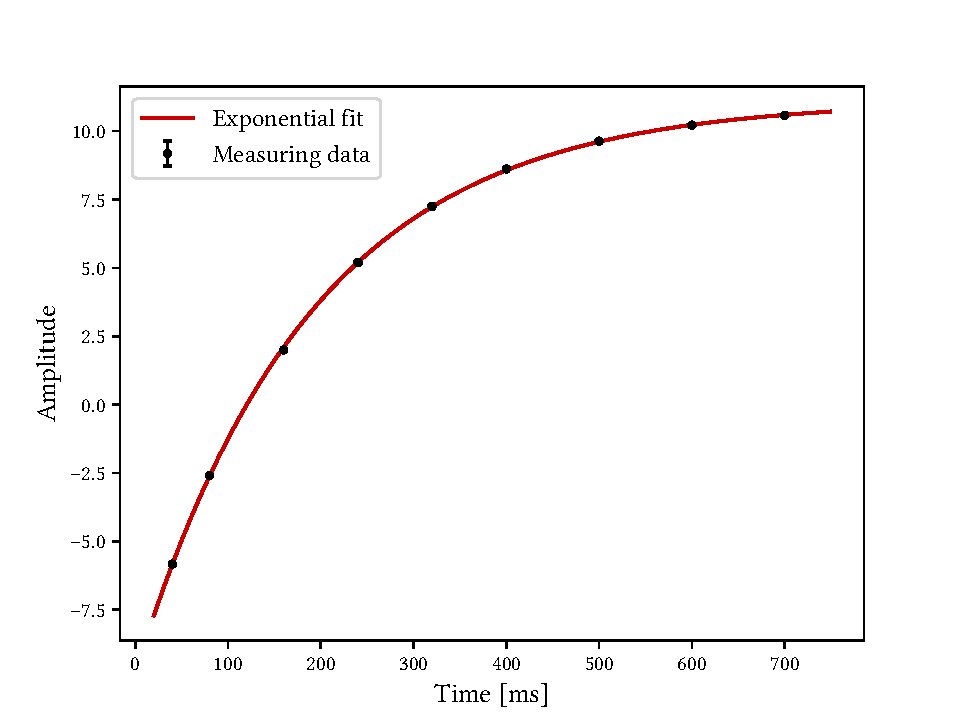
\includegraphics[width=9.3cm]{..//figures//f61_abb_1.pdf}
\caption{Gd500}
\end{subfigure}
\qquad
\begin{subfigure}{.45\textwidth}
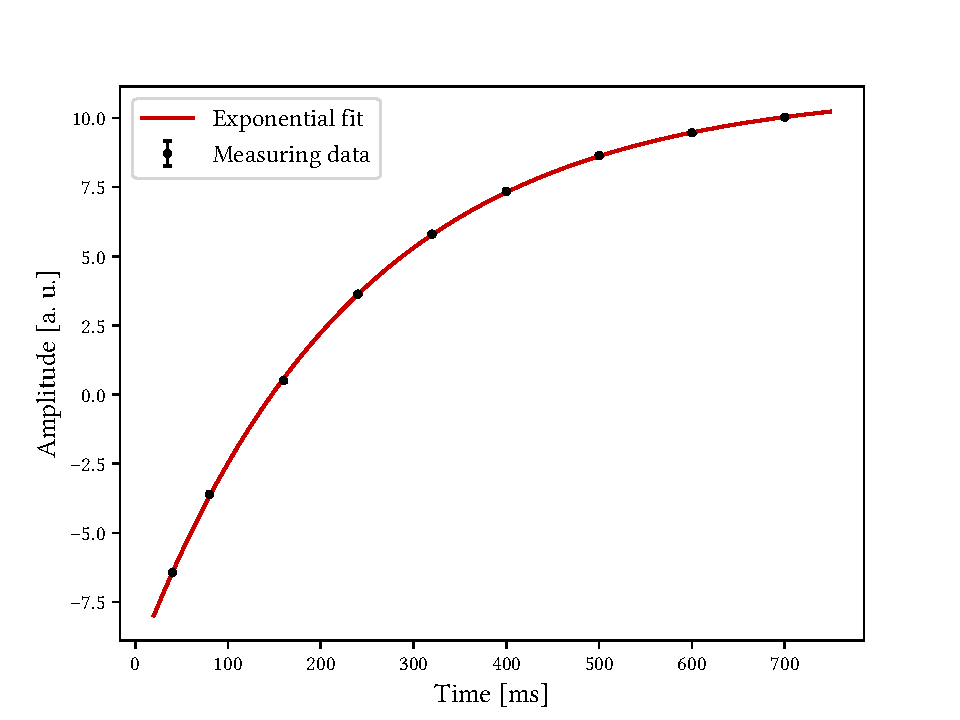
\includegraphics[width=9.3cm]{..//figures//f61_abb_1_600.pdf}
\caption{Gd600}
\end{subfigure}
\caption{Results of the measurement for relaxation time $T_1$.}
\label{fig:t1}
\end{figure}
With the help of Python, an exponential fit according to equation \ref{eq:t1} gives the values
\begin{align*}
T_{1,\text{ Gd500}}&=\SI{190.0(6)}{\milli\second},\\
T_{1,\text{ Gd600}}&=\SI{234.3(5)}{\milli\second}.
\end{align*}

Table \ref{tab:relax} summarizes all three measured relaxation time values for both samples.
\begin{table}[ht]
\centering
\begin{tabular}{cccc}
\toprule
Sample & $T_1$ [ms] & $T_{2,\text{ spin-echo}}$ [ms] & $T_{2,\text{ Carr-Purcell}}$ [ms]\\
\midrule
Gd500 & \num{190.0(6)} & \num{154.2(9)} & \num{170.1(4)}\\
Gd600 & \num{234.3(5)} & \num{186.5(9)} & \num{198.2(7)}\\
\bottomrule
\end{tabular}
\caption{Measured relaxation time.}
\label{tab:relax}
\end{table}
We see that all relaxation times for the more diluted sample Gd600 are longer than with Gd500.
This results directly from the lower Gadolinium content because Gadolinium reduces the relaxation time.\\
Within the measurements of a sample we also see that the spin-echo method delivers shorter times than the Carr-Purcell method.
This is due to the longer recording time of the spin-echo method, in which the sample has time for diffusion and the magnetic field can change.\\
The relaxation time $T_2$ of spin-spin interaction is less than that of spin-lattice $T_1$, because the latter includes the energy release into the environment, while the spin-spin interaction only takes into account the behavior within the molecules.
In general, the theoretical prediction
\begin{align}
T_1\geq T_2
\end{align}
can be determined. 
In order to release energy into the environment, however, it requires a certain threshold value that is higher than that required to perform a spinflip in the molecules.
Therefore, the time for the spin-lattice interaction is longer than for the spin-spin interaction. 



%-----------------------
\subsection{Chemical shift}
In this part of the experiment we measured the Larmor frequencies of unknown substances with and without the reference substance TMS.
This was done by measuring the resonance peaks of the Fourier transform of the registered signal.
We can measure a signal in the frequency spectrum from \num{200} to \SI{900}{\hertz}, which is determined by our magnet.
If we also use pressure air to put our probe into rotation, the width of the frequency response becomes smaller.
\begin{figure}[ht]
\begin{subfigure}{.45\textwidth}
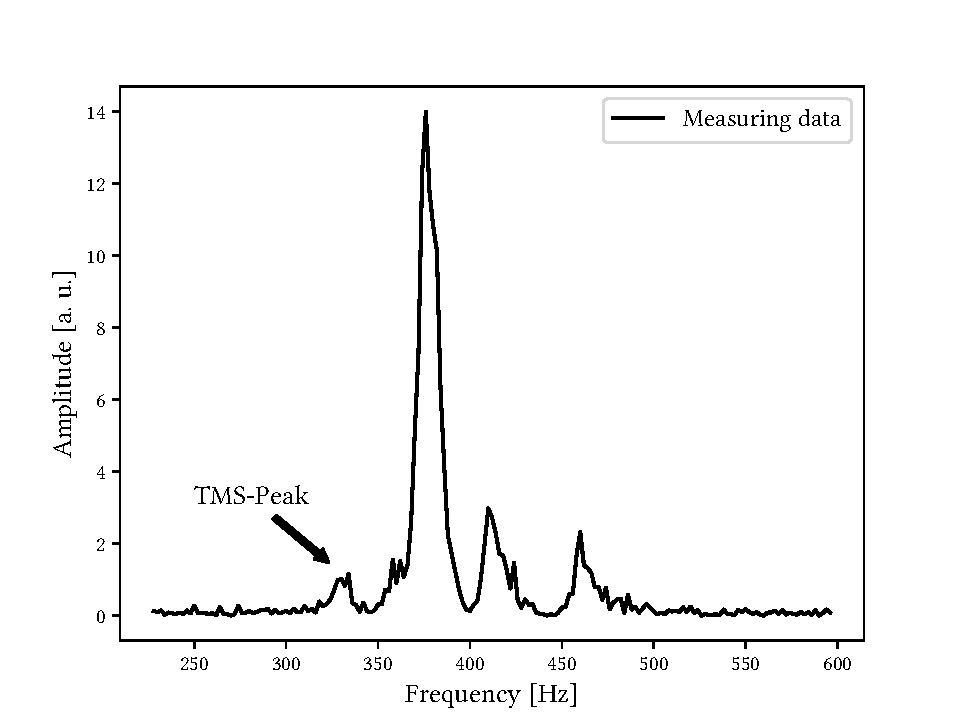
\includegraphics[width=9.3cm]{..//figures//f61_abb_4.pdf}
\caption{Sample A}
\end{subfigure}
\qquad
\begin{subfigure}{.495\textwidth}
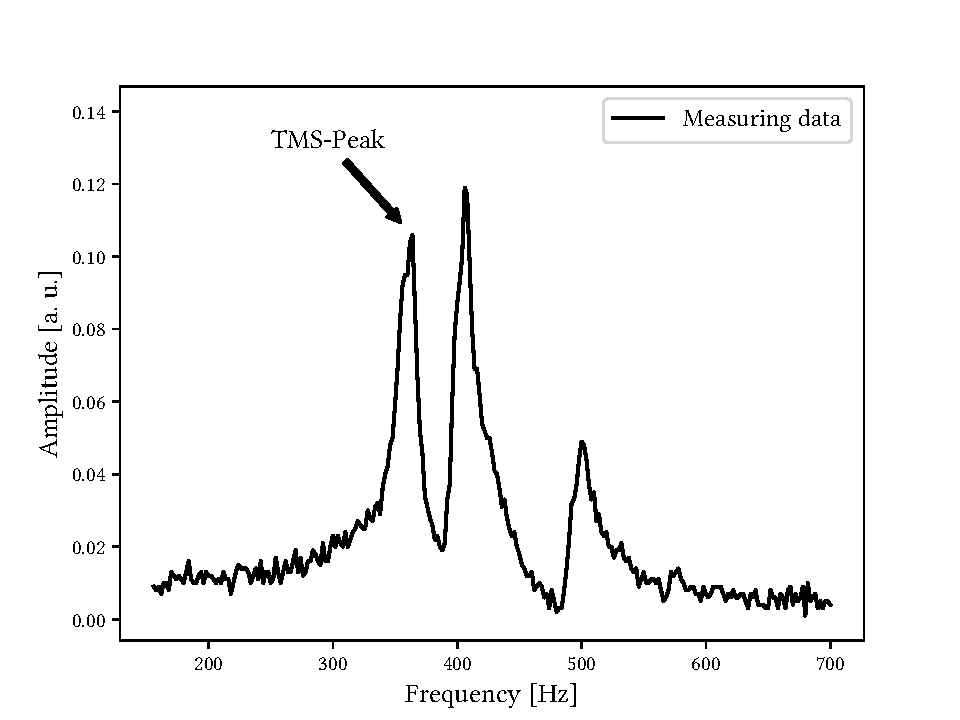
\includegraphics[width=9.3cm]{..//figures//f61_abb_5.pdf}
\caption{Sample B}
\end{subfigure}
\qquad
\begin{subfigure}{.45\textwidth}
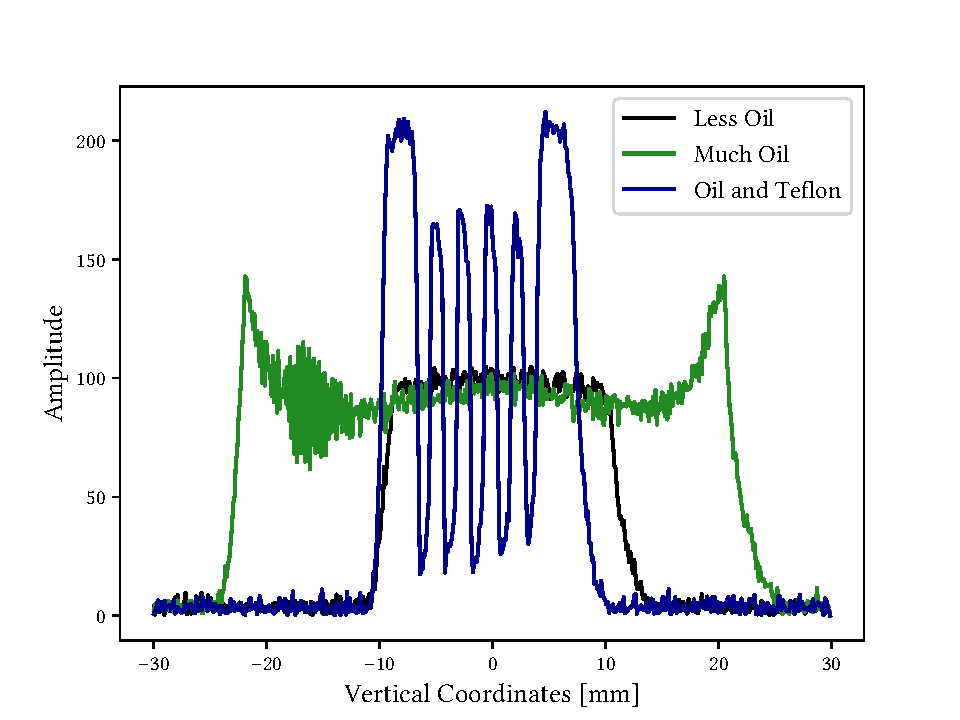
\includegraphics[width=9.3cm]{..//figures//f61_abb_6.pdf}
\caption{Sample C}
\end{subfigure}
\qquad
\begin{subfigure}{.45\textwidth}
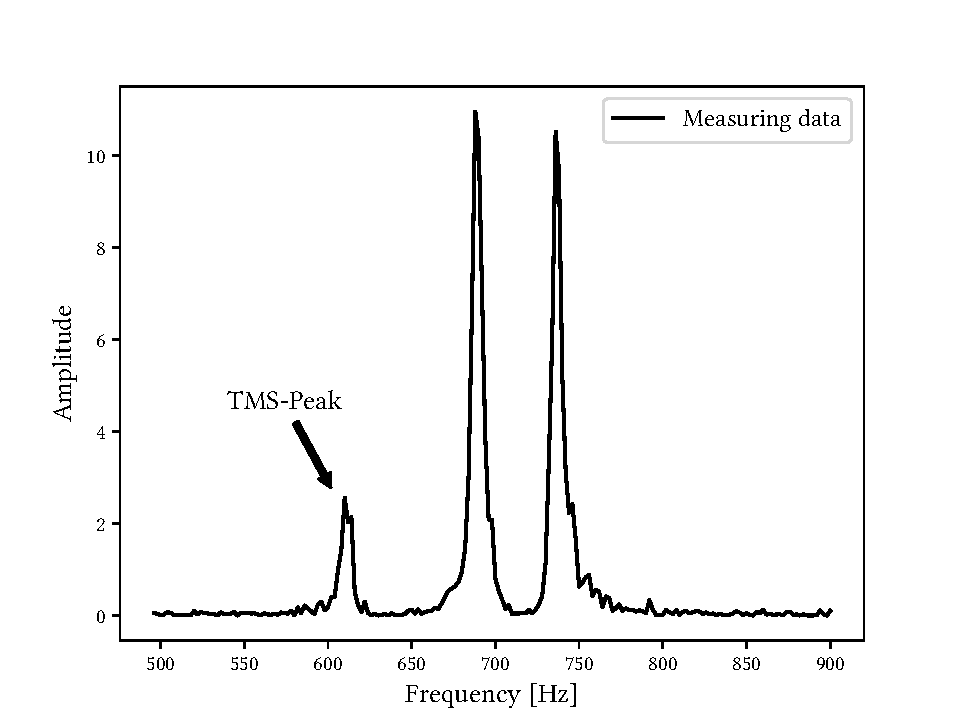
\includegraphics[width=9.3cm]{..//figures//f61_abb_7.pdf}
\caption{Sample D}
\end{subfigure}
\caption{Fourier transform of the registered signal.}
\label{fig:fourier}
\end{figure}
From the frequency shift measured in this way, the chemical shift can be calculated using equation \ref{eq:shift}.
\begin{table}[ht]
\centering
\begin{tabular}{cccccc}
\toprule
Sample & Shift 1 [ppm] & Shift 2 [ppm] & Shift 3 [ppm] & Substance\\
\midrule
A & \num{2.4(1)} & \num{3.9(1)} & \num{6.3(1)} & fluoroacetone\\
B & \num{2.1(1)} & \num{6.9(1)} & & p-xylol\\
C & \num{9.6(1)} & \num{12.0(1)} & & acetic acid\\
D & \num{4.0(1)} & \num{6.4(1)} & & fluoroacetonitril\\
E & \num{2.2(1)} & \num{7.3(1)} & & tuluol\\
\bottomrule
\end{tabular}
\caption{Measured chemical shifts.}
\label{tab:shift}
\end{table}

Experimentally, we had to give a pulse to the magnet every three seconds and continuously adjust the main magnetic field so that the working frequency is around $\nu_\text{w}=\SI{500}{\hertz}$.
Therefore, one wavelength had to be \SI{2}{\milli\second} long, which we could achieve via the screw on the magnet.\\
Table \ref{tab:shift} lists the measured chemical shifts of the different samples and their assignment to the corresponding chemical elements.
Due to missing samples A,D and E, the shifts could unfortunately only be taken over by leading test participants.\\

Now we knew that the elements toluol (CH$_3$ - C$_6$H$_5$), p-xylol (CH$_3$ - C$_6$H$_4$ - CH$_3$), acetic acid (CH$_3$ - COOH), fluoroacetone (FCH$_2$ - CO - CH$_3$) and fluoroacetonitril (FCH$_2$ - CN) were among the samples and could classify them according to the same principle with figure \ref{fig:shift}.\\
Sample C is the only one that has a shift above 10 ppm and therefore must have a COOH group, which only applies to acetic acid.
The two shifts of samples B and E are in fact the same.
The same functional groups, a carbon ring and one or two methyl groups for tuluol and p-xylol, cause the same shifts.
Because p-xylol contains twice the amount of methyl groups, this substance should show a higher ratio in the peak heights.
Sample B shows exactly such a difference and is therefore p-xylol, while sample E is then tuluol.
Both fluoroacetone and fluoroacetonitril have a fluoromethyl group and show two identical shifts.
Nevertheless, the former has a third shift exactly the same size as tuluol and p-xylol, which could be assigned to the simple methyl group.
Therefore, sample A with the additional peak corresponds to fluoroacetone and sample D to fluoroacetonitril.


%--------------------------
\subsection{Imaging techniques}
The following part for the one and two dimensional imaging was performed with a Bruker NMR analyzer mq7. 5 and evaluated with software provided by Bruker.
%--------------------------
\subsubsection{One dimensional imaging}
First we examined the paintings of different heights of oil, as well as when Teflon layers are between the oil.
\begin{figure}[ht]
\centering
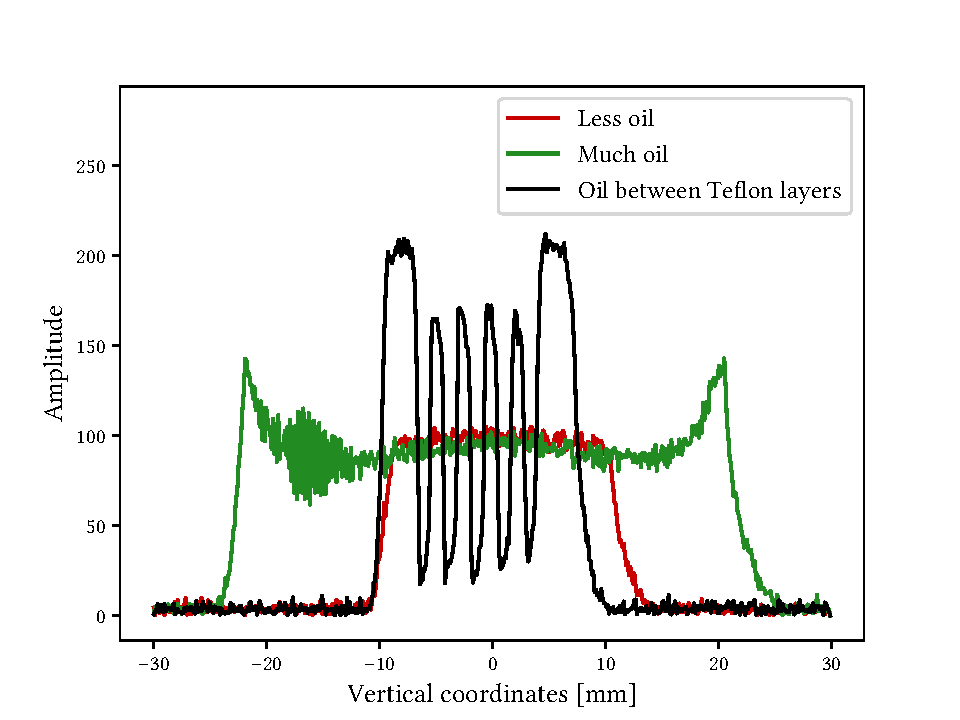
\includegraphics[scale=.6]{..//figures//f61_abb_8.pdf}
\caption{Various oil samples.}
\label{fig:oil}
\end{figure}
Figure \ref{fig:oil} shows very well the structural resolution of the NMR technology.\\
Since the analyzer used is calibrated for hydrogen, we expect signals proportional to the hydrogen density.
For oil this corresponds to a square-wave signal, while Teflon consists of C$_2$F$_4$ units and is therefore not excited.\\
At first glance you can see that the red curve only has a small but constantly wide peak for the small oil content.
On the other hand, the green curve for the large amount of oil at both ends is increased again because the range of the homogeneous magnetic field ends.
In the black curve, the individual Teflon layers, which cannot be detected in the NMR and therefore have no amplitude, can be easily recognized again.\\

Furthermore, we filled a test tube up to about 2 cm with sand and poured oil over it.
\begin{figure}[ht]
\centering
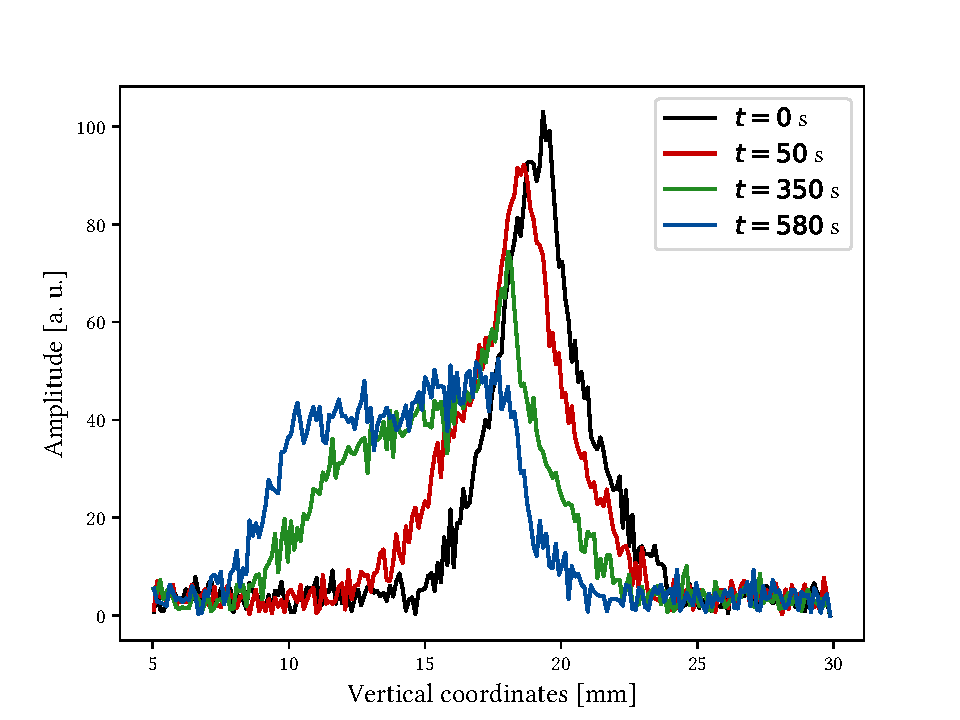
\includegraphics[scale=.6]{..//figures//f61_abb_9.pdf}
\caption{Seepage process of oil in sand (starts with black and ends with brown).}
\label{fig:sand}
\end{figure}
Now we have made regular scans to investigate the seepage process (see fig. \ref{fig:sand}).\\
The question of whether this is diffusion can be answered with the help of Fick's Law
\begin{align}
\pdv{c}{t}=D\pdv[2]{c}{x}
\end{align}
where $c$ is the concentration, $t$ the time, $D$ the diffusion coefficient and $x$ the positive length.\\
The solution of the fuck law tells us that areas with little oil must be filled slowly with individual oil droplets.
This is not the case in the figure, because the fall of the curves is usually too strong at the edges.
Furthermore, a diffusion process must run in negative and positive $x$ direction, which is clearly not the case in our experiment.
It is therefore not a diffusion process.
This is also easy to understand, because besides Brown's molecular movement, gravity also acts as a driving force.
Diffusion has a minor role in this experiment as you can see sometimes an asymptotic decrease.
%---------------------------
\subsubsection{Two dimensional imaging}
In the last part of the experiment some organic substances were analysed in the test tube, this time two dimensional cross-sections were recorded.
Areas in which water is contained produce a stronger signal.
So, in figure \ref{fig:olive} we well learn, that in an olive kernel there is also a liquid.
The air pockets in the peanut are also clearly visible.
But we have also noticed that the correct positioning of the sample plays an enormous role and thus quickly involves a great deal of time.
\begin{figure}[ht]
\begin{subfigure}{.3\textwidth}
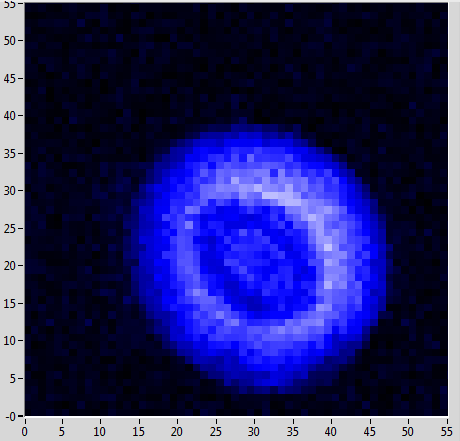
\includegraphics[width=5cm]{..//figures//olive.png}
\caption{Olive}
\label{fig:olive}
\end{subfigure}
\qquad
\begin{subfigure}{.3\textwidth}
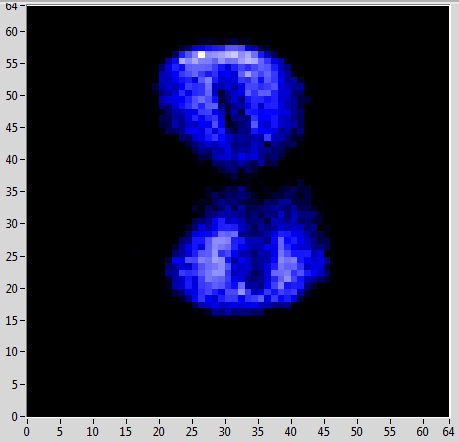
\includegraphics[width=5cm]{..//figures//peanut.png}
\caption{Peanut}
\label{fig:peanut}
\end{subfigure}
\qquad
\begin{subfigure}{.3\textwidth}
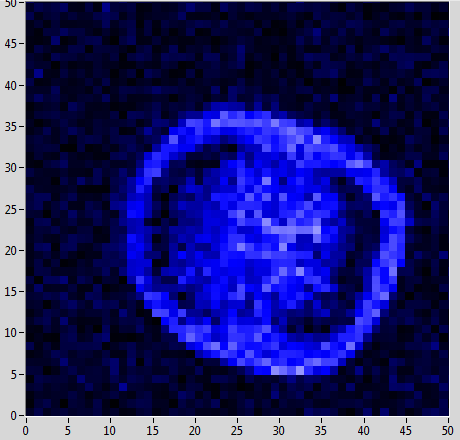
\includegraphics[width=5cm]{..//figures//chilipepper.png}
\caption{Chilipepper}
\end{subfigure}
\caption{Two dimensional NMR imaging.}
\label{fig:2d}
\end{figure}